%% LyX 2.0.8.1 created this file.  For more info, see http://www.lyx.org/.
%% Do not edit unless you really know what you are doing.
\documentclass[english]{article}
\usepackage[T1]{fontenc}
\usepackage[latin9]{inputenc}
\usepackage{float}
\usepackage{graphicx}

\makeatletter
%%%%%%%%%%%%%%%%%%%%%%%%%%%%%% User specified LaTeX commands.
\usepackage{inputenc}
\usepackage{authblk}
% Use only LaTeX2e, calling the article.cls class and 12-point type.



% Users of the {thebibliography} environment or BibTeX should use the
% scicite.sty package, downloadable from *Science* at
% www.sciencemag.org/about/authors/prep/TeX_help/ .
% This package should properly format in-text
% reference calls and reference-list numbers.

\usepackage{cite}

% Use times if you have the font installed; otherwise, comment out the
% following line.

\usepackage{times}

% The preamble here sets up a lot of new/revised commands and
% environments.  It's annoying, but please do *not* try to strip these
% out into a separate .sty file (which could lead to the loss of some
% information when we convert the file to other formats).  Instead, keep
% them in the preamble of your main LaTeX source file.


% The following parameters seem to provide a reasonable page setup.

\topmargin 0.0cm
\oddsidemargin 0.2cm
\textwidth 16cm 
\textheight 21cm
\footskip 1.0cm


%The next command sets up an environment for the abstract to your paper.

\newenvironment{sciabstract}{%
\begin{quote} \bf}{\end{quote}}


% If your reference list includes text notes as well as references,
% include the following line; otherwise, comment it out.

\renewcommand{\refname}{References and Notes}

% The following lines set up an environment for the last note in the
% reference list, which commonly includes acknowledgments of funding,
% help, etc.  It's intended for users of BibTeX or the {thebibliography}
% environment.  Users who are hand-coding their references at the end
% using a list environment such as {enumerate} can simply add another
% item at the end, and it will be numbered automatically.

\newcounter{lastnote}
\newenvironment{scilastnote}{%
\setcounter{lastnote}{\value{enumiv}}%
\addtocounter{lastnote}{+1}%
\begin{list}%
{\arabic{lastnote}.}
{\setlength{\leftmargin}{.22in}}
{\setlength{\labelsep}{.5em}}}{\end{list}}


% Include your paper's title here

\title{Estimating Drivers Cell State Transitions using Gene Regulatory Network Models} 

\makeatother

\usepackage{babel}
\begin{document}

\title{Estimating Drivers Cell State Transitions using Gene Regulatory Network
Models\author[1]{Daniel Schlauch} 
\author[2,3]{Kimberly Glass} 
\author[1,3]{John Quackenbush} 
\affil[1]{Department of Biostatistics and Computational Biology, Dana-Farber Cancer Institute and Department of Biostatistics, Harvard TH Chan School of Public Health, Boston, MA 02115}
\affil[2]{Channing Division of Network Medicine, Brigham and Women's Hospital, Boston, MA 02115}
\affil[3]{Department of Medicine, Harvard Medical School, Boston, MA 02115}}
\maketitle
\begin{abstract}
In the language of systems biology, the state of a cell can be represented
by a gene regulatory network that characterizes the gene transcriptional
processes that are active in that cell type. And transitions that
occur in a wide range of biological processes, ranging from development
to disease, can be thought of as transformation of the gene regulatory
network from its initial state to its final state. Here we propose
a regression-based generalization of the PANDA method for gene regulatory
network inference for individual states, and a regression approach
to modeling cell state transitions, identifying transcription factors
that alter the network structure as cell states change. Our results
demonstrate the ability to find strong signals which persists across
studies and tissues of the same disease and which are not detectable
with conventional gene expression analysis.
\end{abstract}

\section*{Introduction}

One of the fundamental problems is biology is modeling the transition
between biological states such as that which occurs during development
or as a healthy tissue transforms into a disease state. While it is
appealing to conceive of this process as deterministic, reflecting
a change from one well-defined phenotype to another, in truth the
situation is much more complex. Neither the initial nor the final
phenotype is discrete, but each falls into a continuum of states,
which, on average, captures features of that phenotype \textbf{{[}many
citations, too general?{]}}. Indeed, within each tissue there are
many, many cells, each of which is its own particular instance of
that tissue\textemdash{}with unique patterns of gene expression and
individual regulatory processes\cite{mohanty2014model,hu2013heterogeneity}.
The same is true when considering individuals as each healthy and
disease state is unique to each member of a study population. One
way to conceptualize the state transition problem is to imagine that
each phenotype has a characteristic gene regulatory network and that
there are a set of processes that are either activated or inactivated
to transform the network in the initial state into that characterizing
the final state. Identifying those changes could, in principle, help
us to understand not only the processes that drive the state change,
but also how one might intervene to either promote or inhibit such
a transition.

As our ability to generate large-scale integrative multi-omic datasets,
such as RNA-Seq \cite{licatalosi2010rna} and whole genome sequencing,
has grown, there has been an increased interest in using those data
to infer gene regulatory networks to model fundamental biological
processes. While there have been many network inference (NI) methods
published utilizing gene expression or a combination of gene expression\cite{margolin2006aracne, marbach2012wisdom, wille2004sparse, faith2007large, zhang2005general}
and complementary 'Omics data \cite{ernst2008semi,glass2013passing, hecker2009gene},
each of which uses a different approach to estimating the \textquotedblleft{}strength\textquotedblright{}
of interactions between genes (or between transcription factors and
their targets), they all suffer from the same fundamental limitation.
Methods typically rely on estimating weights that represent a measure
of evidence of an interaction between two genes and then setting a
threshold to identify \textquotedblleft{}real\textquotedblright{}
(high confidence) edges. While setting edge confidence thresholds
allows us to graphically represent networks and allows us to compare
networks based on the presence or absence of edges, it ultimately
requires that we discard information regarding those \textquotedblleft{}weak\textquotedblright{}
edges that fail to reach an arbitrary cutoff. Now, one could argue
that discarding low significance edges is sensible as one common goal
in network inference is to deduce a single, high confidence network
model that represents a particular phenotype under study or, in some
cases, a transition between phenotypes. An alternative view is that
these edges contain estimates for gene coexpression that may be muted
due to the heterogeneity of the biological sample and that networks
are best described by edgeweights on a continuous scale. Furthermore,
we argue that the inclusion of all network edgeweights in downstream
analyses allows for the collection of systematic, though subtle, differences
in coexpression which may otherwise have been washed out by extraneous
noise.


\section*{Modeling cell state transitions as a problem in gene regulatory network
transition}

Cell state transitions\textemdash{}such as those that occur during
development, or as healthy tissue transforms into a disease phenotype\textemdash{}are
fundamental properties of biological systems. Understanding what drives
these transitions, and modeling the processes, is one of the great
open challenges in modern biology. One way to conceptualize the state
transition problem is to imagine that each phenotype has its own characteristic
gene regulatory network, and that there are a set of processes that
are either activated or inactivated to transform the network in the
initial state into that which characterizes the final state. Identifying
those changes could, in principle, help us to understand not only
the processes that drive the state change, but also how one might
intervene to either promote or inhibit such a transition. The starting
point for modeling cell state transitions is to model the initial
and final cell states. One might imagine that the initial and final
cell states consist of characteristic processes, some of which are
shared (sometimes referred to as \textquotedblleft{}housekeeping\textquotedblright{}
functions) and others which are unique to the particular state. The
way we understand these processes is that they are controlled by gene
regulatory networks in which transcription factors (and other regulators)
moderate the transcription of individual genes whose expression characterizes
the state. One way to represent such processes is to draw a directed
network graph, in which transcription factors and genes are nodes
network in the network, and edges represent the regulatory interactions
between transcription factors and their target genes that are active
in, and characteristic of, a particular cellular state. One way of
representing such a network, with interactions between m transcription
factors and n target genes, is as a binary $m\times n$ \textquotedblleft{}adjacency
matrix,\textquotedblright{} with 1\textquoteright{}s representing
active transcription factor-target interactions, and 0\textquoteright{}s
representing the lack of a transcription factor-target gene regulatory
interaction. One can then think of a cell fate transition as the process
that transforms the network in its initial state to its final state
form, adding and deleting edges to remake the network that characterizes
one phenotype into that which characterizes the other. Using the adjacency
matrix formalism, one can think of this as a problem in linear algebra
in which we attempt to find an $m\times m$ \textquotedblleft{}transition
matrix\textquotedblright{} $\mathbf{T}$, subject to a set of constraints
that approximates the conversion from the initial network\textquoteright{}s
adjacency matrix \textbf{$\mathbf{A}$} into the final network\textquoteright{}s
adjacency matrix $\mathbf{B}$, or 
\[
\mathbf{B}=\mathbf{AT}
\]


\begin{figure}[h]
\centering{}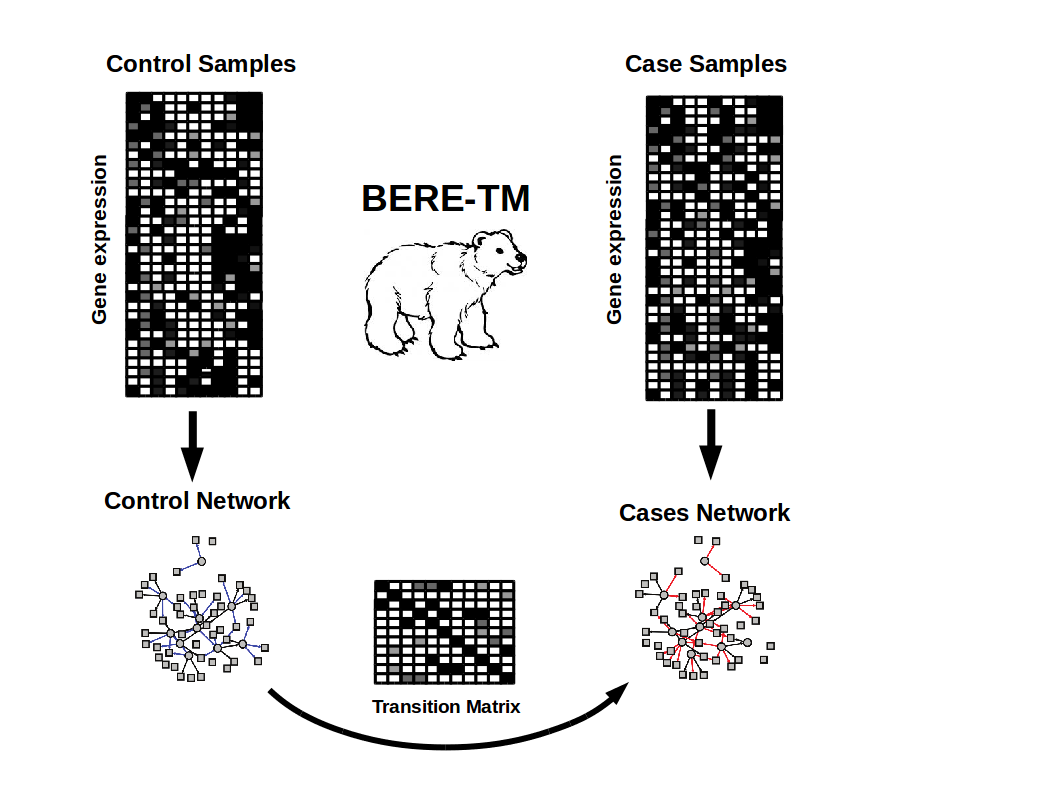
\includegraphics[width=0.5\columnwidth]{figures/figure1_a}\caption{\textbf{Overview of the Transition Matrix problem.} Our approach seeks
to find the $TF\times TF$ matrix which best characterizes the transition
in TF targetting between the regulatory networks of cases and controls.
We can think about this problem as the estimation of the set of TF-TF
interactions which minimizes edgeweight error in the cases network
when applied to the controls network.}
\end{figure}


While it is appealing to conceive of this process as deterministic,
reflecting a change from one well-defined phenotype to another, in
truth the situation is much more complex. Neither the initial nor
the final phenotype is discrete, but each falls into a continuum of
states, which, on average, captures the features of that phenotype.
Indeed, within each tissue there are many, many cells, each of which
is its own particular instance of that tissue\textemdash{}with unique
patterns of gene expression and individual regulatory processes. In
the language of adjacency matrices, what this means is that rather
than representing each state by a matrix with binary entries, what
one should do is use a representation in which entries are continuous,
representing the strength of the transcription factor-target gene
interaction averaged over the collection of samples (or cells) representing
each state. And consequently, the problem of estimating the transition
matrix is generalized to solving $\mathbf{B}=\mathbf{AT}+\mathbf{E}$,
where \textbf{E} is an $m\times n$ error matrix representing unexplained
by our estimated transition and minimized by our procedure. In this
formalism, modeling the cell state transition is equivalent to estimating
the appropriate transition matrix $\mathbf{T}$ that maps how the
transcription factor-target gene interactions are \textquotedblleft{}rewired\textquotedblright{}
between states. And one could hypothesize that the drivers of the
cell state transition are those transcription factors that have the
greatest change in the targets that they regulate.

To generate our gene regulatory networks we are commonly faced with
state-specific gene expression data along with general regulatory
prior knowledge regarding suspected regulatory relationships. {[}BERE-TM
(NAME TBD){]} performs this step by applying a novel, computationally
efficient method which uses each TF's DNA sequence binding motifs
as classifiers for all genes and identifies genes which are coexpressed
with the set of suspected targets as well as removes suspected targets
which do not conform to the TF targets' general pattern of expression
(see supplementary materials and methods). This step yields two $m\times n$
gene regulatory matrices for cases and controls each representing
estimates of the targetting patterns of the $m$ TFs onto the $n$
genes.

Next, the problem is formulated as a regression problem whereby we
solve for the $m\times m$ transition matrix which best describes
the transformation from controls to cases (see supplementary materials
and methods). The $i^{th}$ column in the matrix can be loosely interpreted
as being the optimal linear combination of columns in the controls
adjacency matrix which predict the $i^{th}$ column in the cases adjacency
matrix. Naturally, we expect the transition matrix between two identical
states to approximate the identity matrix. Intuitively, it is the
deviation from the identity matrix which is of biological interest
with off diagonal mass at point $\left(i,j\right)$ indicating a regulatory
alteration between cases and controls involving the $i^{th}$ and
$j^{th}$ TF. Focusing specifically on individual TF behavioral modifications,
one might simply be interested in the overall changes for each column.
This can be obtained via the sum of off-diagonal ``mass'' representing
the sum of systematic modifications estimated in transitioning from
controls to cases. Furthermore, the statistical significance of these
results is estimated by permuting the case-control labels $n$ times
and rerunning the the analysis to determine the proportion of null
results which are more extreme than the observed result (see supplementary
materials and methods).

In evaluating the state transitions, we recognize the limitations
of current network inference methods to predict individual edgeweights
with a high degree of confidence. It's therefore of interest to combine
measurements across sets of edgeweights in order to extract meaningful
signal from a network perturbation. Effectively, we approached the
problem as a dimension reduction problem with the goal of identifying
high-influence, systematic regulatory network alterations rather than
isolated independent events. There are many existing methods for reducing
a high-dimensional matrices which may be applied to a gene regulatory
adjacency matrix. Commonly, Principal Components Analysis (PCA) identifies
eigenvectors which can reconstruct the greatest degree of variance
from the original data. One drawback of this approach is the lack
of interpret-ability of these vectors. Our transition matrix approach
can be considered as a data reduction method which (1) reduces the
dimensionality of the differences between two networks (2) preserves
the intuitive interpretation of its vectors and (3) utilizes our expectation
that meaningful network transitions will occur via biologically systematic
alterations and not via random, independent edge alterations.


\section*{{[}BERE-TM (NAME TBD){]} finds significantly differentially involved
TFs in COPD with strong concordance in independent datasets}

We applied our method to four case-control datasets for Chronic Obstructive
Pulmonary Disease (COPD)- Evaluation of COPD Longitudinally to Identify
Predictive Surrogate Endpoints (ECLIPSE)\cite{vestbo2008evaluation}
(Figure \ref{fig:ECLIPSE_results}) , the COPDGene study \cite{pillai2009genome}
(Supplemental Data), Lung Genomics Research Consortium (LGRC) \cite{lgrc}(Supplemental
Data) and Lung Tissue Chronic Obstructive Pulmonary Disease (LTCOPD)
\cite{ltcopd} (Supplemental Data). Each of these studies consisted
of gene expression assays obtained from patients with COPD and a set
of smoker controls. The tissue used in the ECLIPSE and COPDGene study
was peripheral blood mononuclear cell (PBMC), while lung tissue was
sampled for LGRC and LTCOPD. It is therefore reassuring that agreement
is more strongly achieved between studies of the same tissue origin
than acros tissues. Each of the four studies was most closely correlated
with studies of the same tissue. However it is quite notable that
the we do see much of the same dTFI signal across studies involving
different tissue types. Gene regulatory networks derived from gene
expression data are notoriously difficult to replicate across studies
and it is of great interest that we have identified suspected mechanisms
which are correlated not only across studies but across tissues as
well.

We separately applied our BERE network inference approach on cases
and controls and computed the transition matrix. Top significance
hits for dTFI showed strong concordance between each of the datasets.
Out of 166 TF used in this study, seven were among top 10 most differentially
involved in both the ECLIPSE and COPDGene studies (\inputencoding{latin1}{Figure
}\inputencoding{latin9}\ref{fig:compare}). Furthermore, three of
these seven TFs (GABPA, ELK4, ELK1) also appeared as significant in
the LGRC results with FDR<.01.

\begin{figure}[H]
\textbf{A}

\textbf{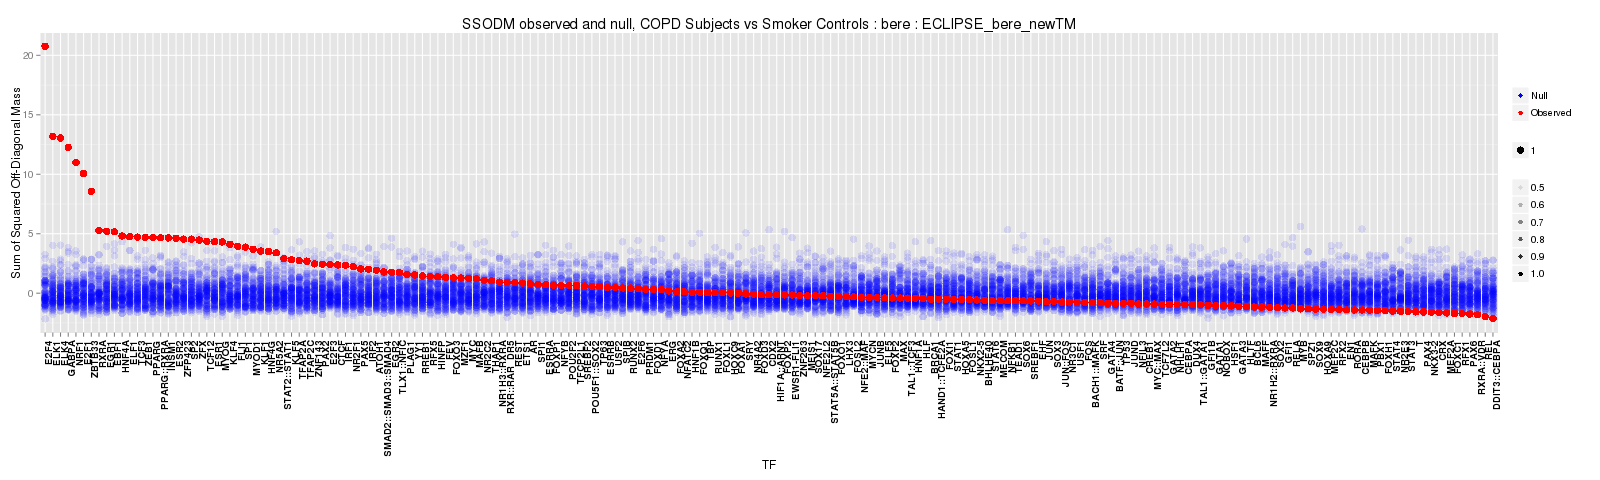
\includegraphics[width=1\columnwidth]{figures/pasted6a}}

\textbf{B}

\textbf{\includegraphics[width=1\columnwidth]{\string"figures/dTFI vs LIMMA55557\string".png}}

\textbf{C}

\includegraphics[width=0.5\columnwidth]{\string"figures/Transition plot55557\string".png}

\caption{\textbf{(A)} \textbf{Differential transcription factor involvement
in ECLIPSE study.} Observed TFs undergoing state transition (red)
scaled for each TF by the distribution under the randomization of
case-control labels (blue). \textbf{(B) Comparison of TF differential
involvement vs differential expression.} TFs which are differentially
involved are not necessarily differentially expressed and vice versa.
Many TFs can be observed which have significantly different targetting
patterns, but which are not statistically significantly differentially
expressed. This suggests that our method finds transcription factors
which are differentially affected at a post-transcription stage. \textbf{(C)
Driver network transitions}. Network transitions are depicted here
with arrows indicating the flow of targetting patterns from one transcription
factor to another. Edges are sized according to the magnitude of the
transition and nodes (TFs) are sized by the overall dTFI for each
TF. The gain of targetting features is indicated by the color blue
while the loss of features is indicated by red.}
\label{fig:ECLIPSE_results}
\end{figure}


Overall, there was a strong correlation between results in the two
PBMC studies $\left(r_{s}=0.87\right)$ and the two lung tissue studies
$\left(r_{s}=0.71\right)$ , and a weaker correlation between cross-tissue
results $\left(\bar{r}_{s}=0.63\right)$.

Of further interest is the particular TFs which are differentially
observed across studies. For example, ERS1, the gene encoding Estrogen
receptor alpha (ES-$\alpha$) is likely to behave differently in males
compared with females. We found that this TF is significantly differentially
involved in the COPDGene study - identified as the $4th$ most differentially
involved TF, but not the ECLIPSE study. Accordingly, the COPDGene
study had a greater gender disparity $\left(\mbox{Odds Ratio}=1.126\right)$
than the ECLIPSE study $\left(\mbox{Odds Ratio}=1.067\right)$.

\begin{figure}[H]
\textbf{A}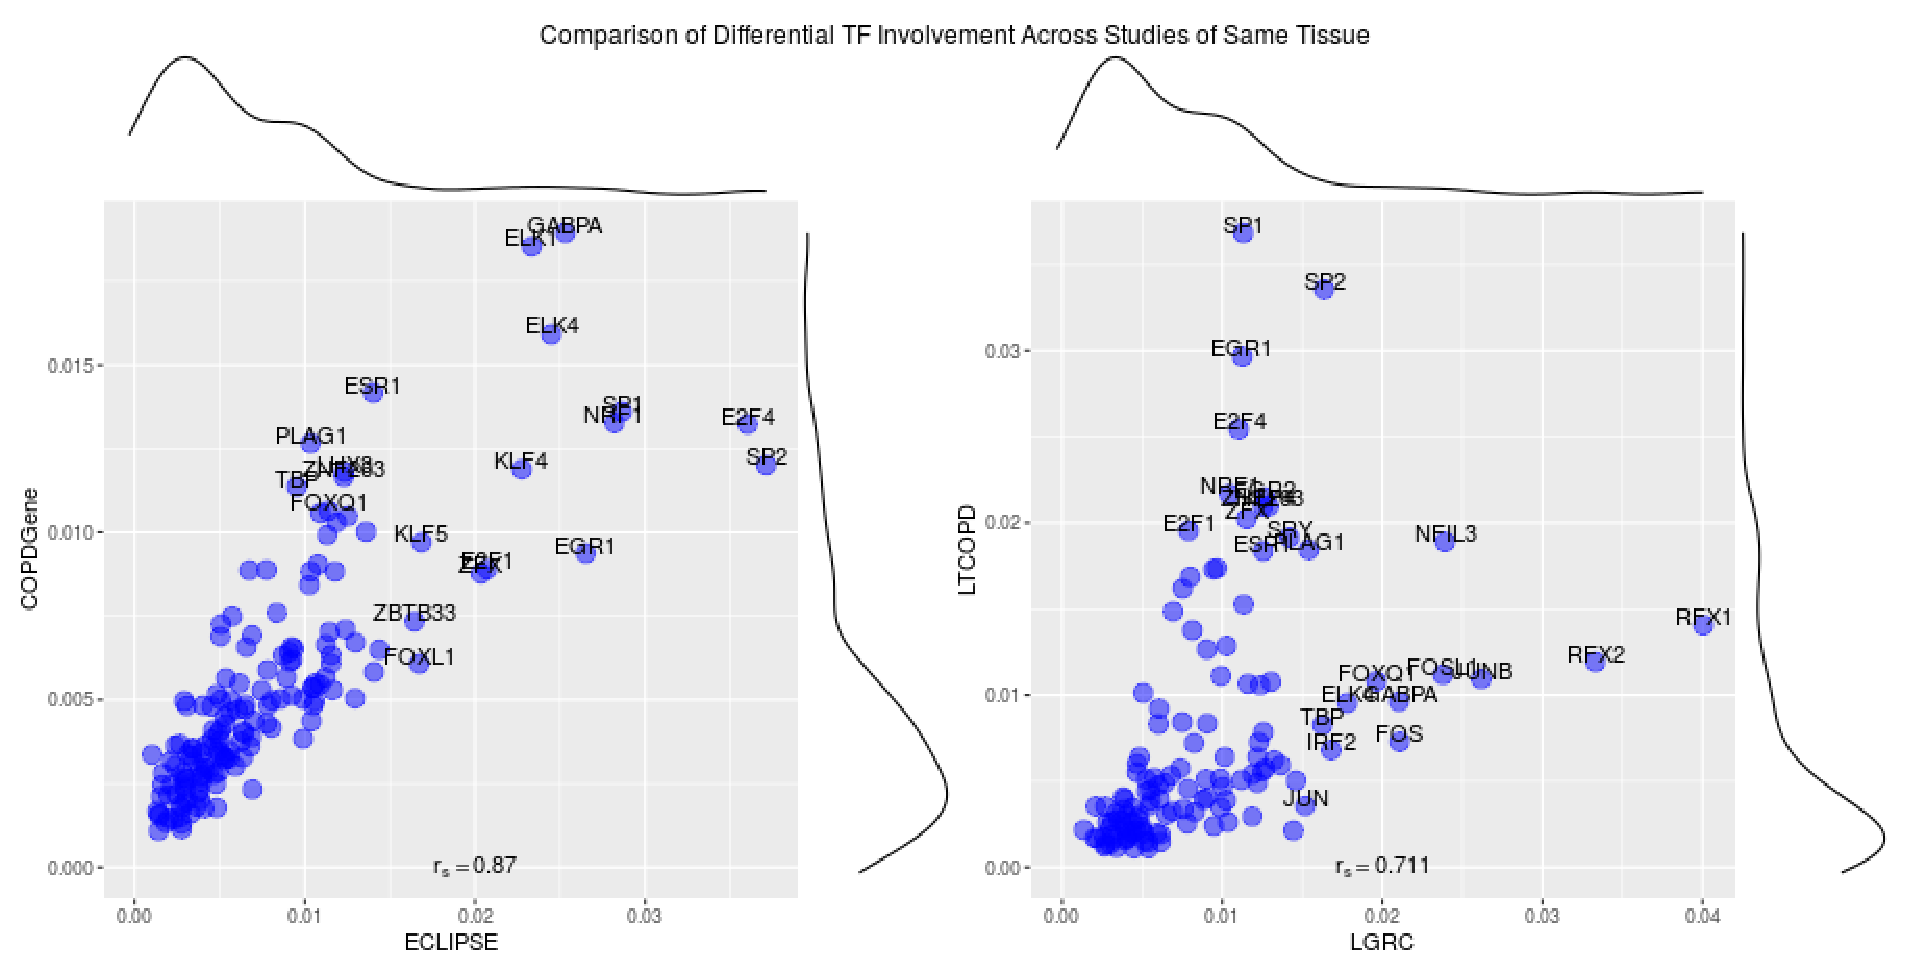
\includegraphics[width=0.6\columnwidth]{figures/eclipse_copdgene_lgrc_comparison_same_tissue}

\textbf{B}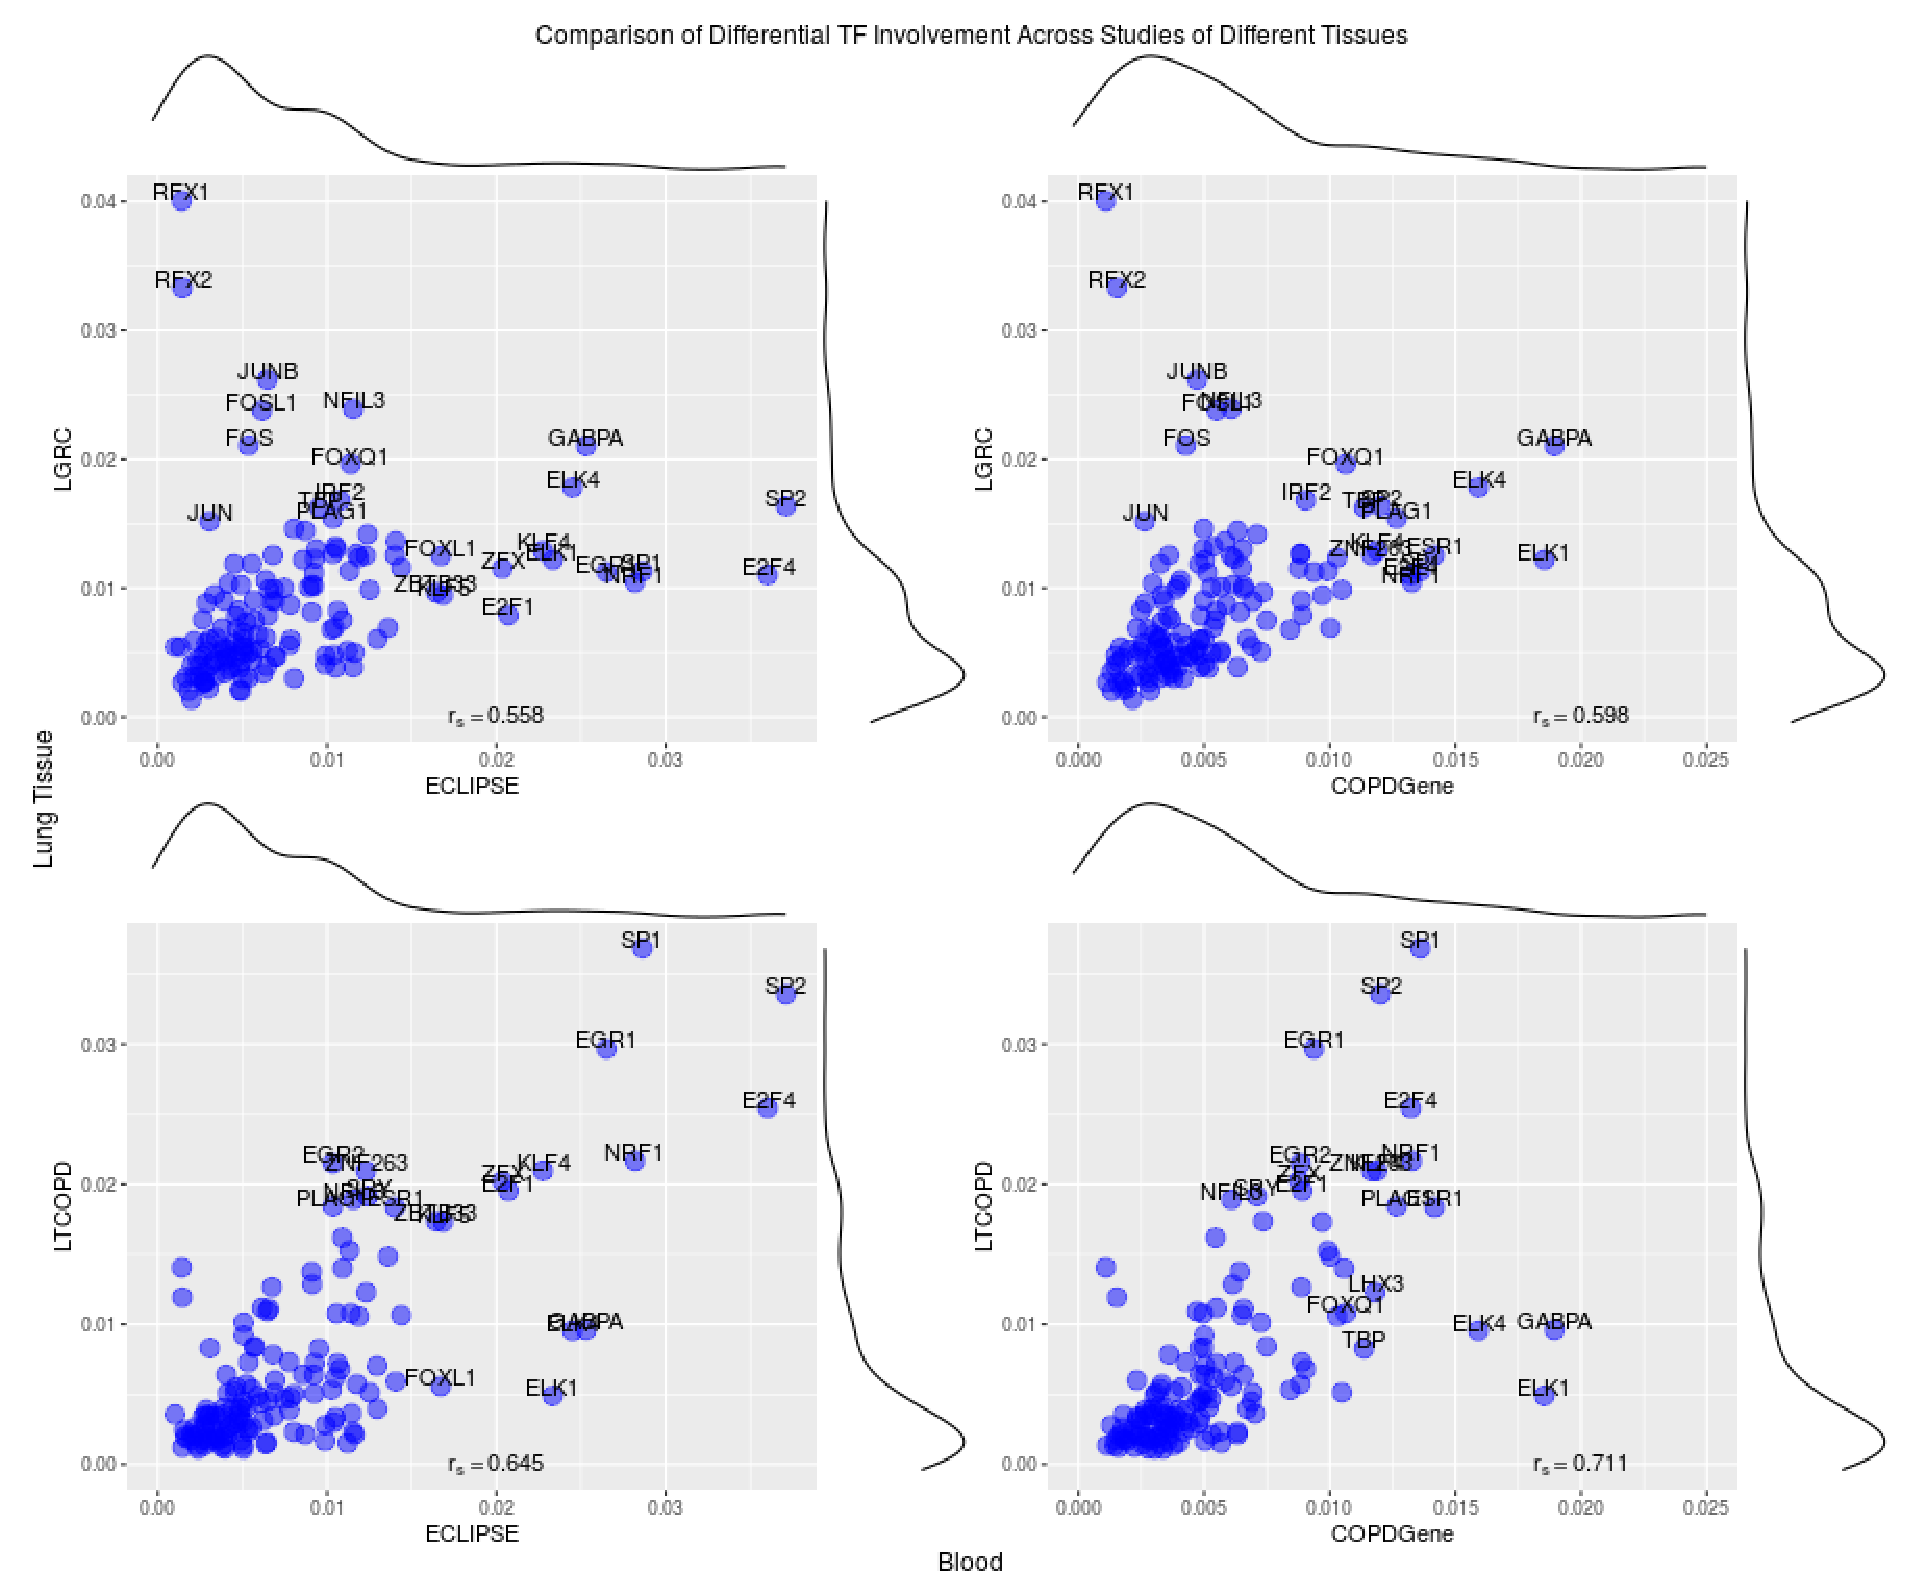
\includegraphics[width=0.6\columnwidth]{figures/eclipse_copdgene_lgrc_comparison_diff_tissue}

\caption{Comparison of dTFI for 166 TFs across four independent studies in
two tissues. ECLIPSE and COPGene data were obtained via PBMC and LGRC
and LTCOPD were obtained via lung tissue. Results for two studies
with gene expression data obtained from the same source (A), PBMC
(left) and lung tissue (right) show strong concordance with a high
degree of agreement, particularly for top hits. Spearman correlation
for each of these tissue types was $r_{s}=.87$ and $r_{s}=.71$,
respectively. Correlations for across tissue study comparisons demonstrated
a weaker, but still measureable agreement. Each of the four studies
was most consistent with the study of the same tissue type as its
own.}
\label{fig:compare}
\end{figure}


Notably in the LGRC dataset, we discovered a differential targetting
pattern involving the TFs RFX1 and RFX2. Both of these transcription
factors were highly statistically significant (FDR<.0001) and ranked
as the top two results in the LGRC study. However, their signal was
muted in the ECLIPSE and COPDGene studies, neither of which identified
these transcription factors as drivers of the Smoker Control to COPD
transition. There are many possible explanations for this result,
but it is reasonable to speculate that the dramatically different
result is due to the fact that the tissue of origin for the LGRC differs
from the ECLIPSE and COPDGene tissue.

The top hits which are most consistent across studies have been implicated
in independent studies for the development of COPD. Two of the top
3 hits, NRF1 and GABPA have been implicated in a mitochondrial mechanism
for disease progression {[}Cloonan, Suzanne M et al{]}. Interestingly,
the majority of the TFs identified as differentially involved do not
exhibit significant differential gene expression. This suggests that
for these proteins, their role in the disease may not occur until
the post-transcription stage. It also suggests that conventional gene
expression analysis is insufficient for identifying many of the TF
drivers of disease.

\bibliographystyle{plain}
\bibliography{./dissertation_research}

\end{document}
